\section{Estados de nodos y red}
El protocolo de comunicación CANae está diseñado para ser sencillo en su uso,
por lo tanto, los nodos como la red pasan por estados de funcionamiento
que son sencillos y atómicos. En esta versión se pretende desarrollar las bases
para los futuros avances sobre el mismo.

En primer lugar el ciclo de vida de un nodo comienza cuando es alimentando. El
nodo empieza en un estado Stand-by hasta que se inicializa internamente. Luego
pasa a un estado de \textit{Waiting Monitor}, donde espera las ordenes de un
\textit{Monitor Node}.  Luego cuando recibe la señales del monitor comienza a
configurarse internamente (ver: \label{Appendix:DBT} y \label{Appendix:NMT}).
Luego de esto pasa a un estado \textit{Working}. Aquí pueden ocurrir dos
situaciones. En primer lugar, el nodo se apaga intencionalmente. La segunda
situación es que el nodo falla y es detectado por el \ac{FDIR}, entonces pasa
a un estado \textit{Failure}.

\begin{figure}[h!]
 \centering
 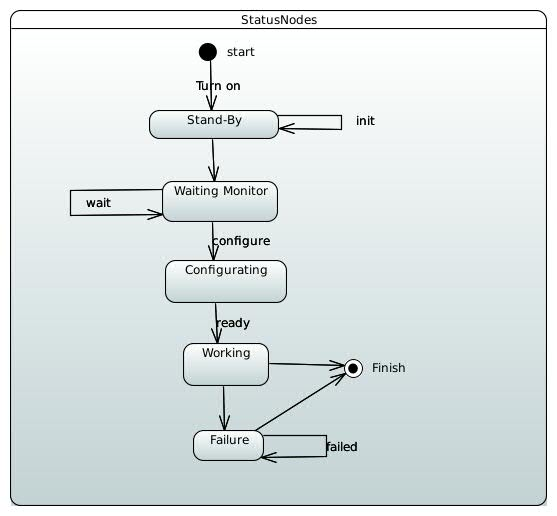
\includegraphics[scale=0.4]{images/Secciones/AppendixA/StatusNode.JPG}
  \caption{Definición de la entidad NMT}
\label{fig:NodeStatus}
\end{figure}

Por otro lado en el entorno de la red CANae, el ciclo de vida de la red comienza
con la alimentación de los nodos. En primer lugar entra en un estado de
\textit{Init Nodes} donde todos los nodos de la red se encuentran desarrollando
su ciclo de vida, tal como se indicó anteriormente. Luego la red pasa a un
estado \textit{Stand-By} para luego comenar el estado de \textit{Creating
  Network}. Dentro de este estado, se dan diferentes estados, se necesita que
todos los nodos se encuentren coordinados. Estos se detallan en
\ref{Appendix:NMT}. Luego de su creación toda la red se encuentra en estado
\textit{Ready} donde se lleva a cabo su normal funcionamiento.

\begin{figure}[h!]
 \centering
 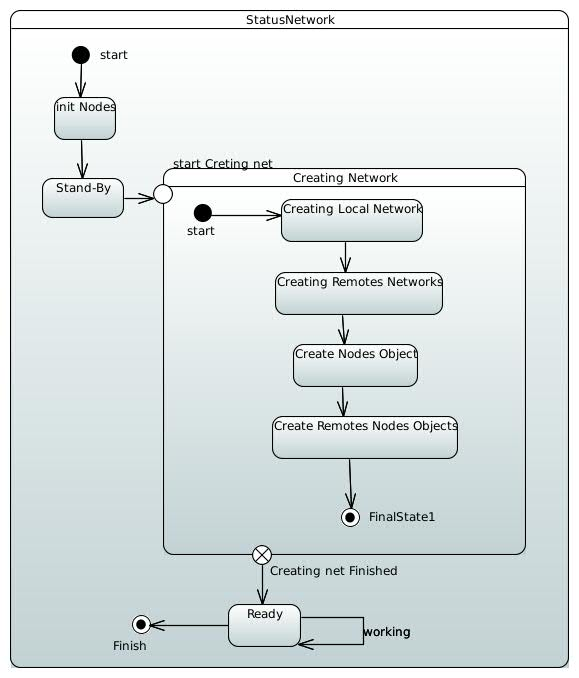
\includegraphics[scale=0.4]{images/Secciones/AppendixA/StatusNetwork.JPG}
  \caption{Definición de la entidad NMT}
\label{fig:NodeStatus}
\end{figure}

